\chapter{Теретические основы кодов, контролирующих ошибки}

В данном разделе приводятся сведения о кодах, контролирующих ошибки, необходимые для дальнейшего изложения
материала.

%%%%%%%%%%%%%%%%%%%%%%%%%%%%%%%%%%%%%%%%%%%%%%%%%%%%%%%%%%%%%%%%%%%%%%%%%%%%%%%%%%%%%%%%%%%
%%%%%%%%%%%%%%%%%%%%%%%%%%%%%%%%%%%%%%%%%%%%%%%%%%%%%%%%%%%%%%%%%%%%%%%%%%%%%%%%%%%%%%%%%%%
%%%%%%%%%%%%%%%%%%%%%%%%%%%%%%%%%%%%%%%%%%%%%%%%%%%%%%%%%%%%%%%%%%%%%%%%%%%%%%%%%%%%%%%%%%%
\section{Блоковые коды}
\begin{definition} 
\deft{Блоковый код} мощности $M$ над алфавитом из $q$ символов --- это множество из $M$ $q$-ичных последовательностей длины $n$, называемых \emph{кодовыми словами}. 
\end{definition}

При $q=2$ символы называются \deft{битами}, а код --- \deft{двоичным}. Как правило, $M=q^k$ для некоторого $k$. Такой код носит название \emph{$(n,k)$-код}. Каждой последовательности из $k$ $q$-ичных символов можно сопоставить последовательность из $n$ $q$-ичных символов, которая и является кодовым словом. Блоковый код задает $n$-символьное кодовое слово, которое включает $k$ информационных символов.

\begin{definition}
\deft{Скорость} блокового кода --- величина $R=k/n$.
\end{definition}

Основные параметры блокового кода:
\begin{enumerate}
\item длина блока $n$
\item информационная длина $k$
\item минимальное расстоянию $d^*$
\end{enumerate}

Минимальное расстояние является мерой различия двух наиболее похожих кодовых слов.

\begin{definition}
\deft{Расстояние по Хеммингу} между двумя $q$-ичными последовательностями $x$ и $y$ длины $n$ --- число позиций, в которых данные последовательности отличаются. Обозначение: $d(x, y)$.
\end{definition}

Пример расстояния, $d(01011, 00111)=2$.

\begin{definition} 
Пусть $\mathfrak{C}=\{c_i, i=0, \ldots, M - 1\}$~---~код. Тогда \deft{минимальное 
расстояние} кода $\mathfrak{C}$ равно наименьшему из всех расстояний по Хеммингу между различными парами 
кодовых слов, т.е. 
$$ d^*  = \mathop {\mathop {\min }\limits_{c_i ,\,c_j  \in \mathfrak{C}} }\limits_{i \ne j}
\left( {c_i ,\;c_j } \right) $$ 
\end{definition}

\begin{definition} 
$(n, k)$-код с минимальным расстоянием $d^*$ называется $(n, k, d^*)$-кодом.
\end{definition}

В случае возникновения в канале $t$ ошибок при передаче кодового слова результат декодирования зависит
от расстояния от принятого слова до каждого другого слова. Так, в случае, если расстояние от принятого
слова до каждого другого кодового слова превосходит $t$, то ошибки будут исправлены, а ближайшее
к принятому кодовое слово будет принято в качестве действительно переданного. Данное утверждение
выполняется только в случае $$d^* \geq 2t+1.$$

%%%%%%%%%%%%%%%%%%%%%%%%%%%%%%%%%%%%%%%%%%%%%%%%%%%%%%%%%%%%%%%%%%%%%%%%%%%%%%%%%%%%%%%%%%%
%%%%%%%%%%%%%%%%%%%%%%%%%%%%%%%%%%%%%%%%%%%%%%%%%%%%%%%%%%%%%%%%%%%%%%%%%%%%%%%%%%%%%%%%%%%
%%%%%%%%%%%%%%%%%%%%%%%%%%%%%%%%%%%%%%%%%%%%%%%%%%%%%%%%%%%%%%%%%%%%%%%%%%%%%%%%%%%%%%%%%%%
\subsection{Линейные блоковые коды}

Большинство известных хороших кодов принадлежат классу \deft{линейных кодов}.

\begin{definition} 
\deft{Линейный код} --- подпространство в векторном пространстве $GF^n(q)$.
\end{definition}

Таким образом, линейный код есть непустое множество $n$-последовательностей над
полем Галуа $GF(q)$. Данные последовательности называемых кодовыми словами. Особенностью множества
является то, что сумма двух кодовых слов является кодовым словом, а произведение любого кодового слова на элемент поля также является кодовым словом.

\begin{definition}
\deft{Систематический код} --- код, у которого всякое кодовое слово начинается с информационных символов. Оставшиеся символы называются \deft{проверочными символами}.
\end{definition}

\begin{definition} \deft{Вес Хемминга $\omega(с)$} кодового слова $c$ --- число ненулевых компонент.
\deft{Минимальный вес кода $\omega^*$} --- минимальный вес ненулевого кодового слова.
\end{definition}

\begin{theorem} 
Для линейного кода минимальное расстояние $d^*$ равно минимальному весу $\omega^*$.
\end{theorem}

\begin{theorem} 
Минимальное расстояние любого линейного $(n, k)$-кода удовлетворяет неравенству $$d^* \leq 1+n-k.$$
\end{theorem}

\begin{definition}
Любой $(n, k)$-код с минимальным расстоянием, которое удовлетворяет равенству $$d^*=1+n-k$$ называется
\deft{кодом с максимальным расстоянием}.
\end{definition}

Согласно Границе Синглтона для исправления $t$ ошибок код должен иметь не менее $2t$ проверочных
символов (2 проверочных символа на ошибку). Коды с максимальным расстоянием имеют точно $2t$
проверочных символов.

%%%%%%%%%%%%%%%%%%%%%%%%%%%%%%%%%%%%%%%%%%%%%%%%%%%%%%%%%%%%%%%%%%%%%%%%%%%%%%%%%%%%%%%%%%%
%%%%%%%%%%%%%%%%%%%%%%%%%%%%%%%%%%%%%%%%%%%%%%%%%%%%%%%%%%%%%%%%%%%%%%%%%%%%%%%%%%%%%%%%%%%
%%%%%%%%%%%%%%%%%%%%%%%%%%%%%%%%%%%%%%%%%%%%%%%%%%%%%%%%%%%%%%%%%%%%%%%%%%%%%%%%%%%%%%%%%%%
\subsection{Циклические коды}
Циклические коды составляют относительно большую группу наиболее широко используемых на 
практике линейных систематических кодов. Их основное свойство, давшее им название, 
заключается в том, что каждый вектор, получаемый из исходного кодового вектора путем 
циклической перестановки его символов, также является разрешенным кодовым вектором.
В качестве математического аппарата для построения данных кодов используется теория полей Галуа.

Операции кодирования и декодирования циклических кодов сводятся к известным процедурам 
умножения и деления полиномов. Для двоичных кодов эти операции легко реализуются 
технически с помощью линейных переключательных схем (ЛПС), при этом получаются 
относительно простые схемы кодеков, в чем состоит одно из практических достоинств циклических кодов.

\begin{definition}
Линейный $(n, k)$-код $\mathfrak{C}$ называется \deft{циклическим}, если
из того, что слово $c=(c_0, c_1, \ldots, c_{n-1})$ принадлежит коду $\mathfrak{C}$,
следует, что слово $c^\prime=(c_{n-1}, c_0, c_1, \ldots, c_{n-2})$ также принадлежит
коду $\mathfrak{C}$.
\end{definition}

Кодовое слово $c^\prime$ получается циклическим сдвигом всех компонент слова $c$ вправо
на одну позицию. Каждый линейный код над $GF(q)$ длины $n$ представляет собой
подпространство пространства $GF^n(q)$, а циклический код является частным случаем
подпространства, так как обладает дополнительным свойством цикличности.

Каждый вектор из $GF^n(q)$ можно представить многочленом от $x$ степени не выше $n-1$. Компоненты вектора 
отождествляются с коэффициентами многочлена. Множество многочленов обладает структурой векторного 
пространства, идентичной структуре пространства $GF^n(q)$. Это же множество многочленов обладает структурой 
кольца $GF(q)[x]/(x^n-1)$. Как в кольце, в этом множестве определено умножение $$p_1(x)\cdot p_2(x)=R_{x^n-1} 
\left[{p_1(x)p_2(x)}\right]$$ где $R_{h(x)}\left[{f(x)g(x)}\right]$~---~есть остаток от деления на многочлен $
 h(x)$ произведения многочленов $f(x)$ и $g(x)$. Заметим, что в приведенное равенство входят произведения 
двух видов. Произведение в левой части является произведением в кольце $GF(q)[x]/(x^n-1)$, определенным через 
произведения к кольце $GF(q)[x]$ в правой части. Циклический сдвиг может быть записан через умножение в этом 
кольце: $$x\cdot p(x)=R_{x^n-1}[xp(x)].$$

Итак, если кодовые слова некоторого кода задаются в виде многочленов, то код является подмножеством
кольца $GF(q)[x]/(x^n-1)$. Такой код является циклическим, если вместе с каждым кодовым словом $c(x)$
он содержит кодовый многочлен $x\cdot c(x)$.

\begin{definition}
\deft{Порождающий многочленом} кода $\mathfrak{C}$ --- единственный приведенный ненулевой многочлен наименьшей степени в коде $\mathfrak{C}$. Обозначение: $g(x)$.
\end{definition}

\begin{theorem} 
Циклический $(n, k)$-код состоит из всех произведений порождающего многочлена $g(x)$ степени $n-k$ на многочлены степени не выше $k-1$.
\end{theorem}

\begin{theorem}
\label{th5.2.3} Циклический код длины $n$ с порождающим многочленом $g(x)$ существует тогда
и только тогда, когда $g(x)$ делит $x^n-1$.
\end{theorem}

Согласно теореме \ref{th5.2.3}, для порождающего многочлена $g(x)$ любого циклического кода выполняется 
равенство $$x^n-1=g(x)h(x)$$ при некотором многочлене $h(x)$. Многочлен $h(x)$ называется \deft{проверочным 
многочленом}. Каждое кодовое слово $c(x)$ удовлетворяет равенству $$R_{x^n-1}[h(x)c(x)]=0.$$

Пусть $c(x)$ обозначает переданное кодовое слово. Это значит что символами переданного слова были 
коэффициенты многочлена $c(x)$. Пусть многочлен $v(x)$ обозначает принятое слово, и пусть $e(x)=v(x)-c(x)$. 
Многочлен $e(x)$ называется \deft{многочленом ошибок}. Ненулевые коэффициенты этого многочлена стоят в тех 
позициях, где в канале произошли ошибки.

Представим информационную последовательность в виде многочлена $i(x)$ степени не выше $k-1$. Множество 
информационных многочленов можно отобразить в кодовые многочлены многими способами. Одним простым правилом 
является $$c(x)=i(x)g(x).$$

Такой кодер является несистематическим, так как по многочлену $c(x)$ нельзя сразу установить $i(x)$. 
Систематическое правило кодирования имеет следующий вид: $$c(x)=x^{n-k}i(x)+t(x),$$ где $t(x)=-R_{g(x)}\left[x
^{n-k}i(x)\right]$.

И систематическое, и несистематическое правила кодирования дают одно и тоже множество кодовых слов, но 
соответствия между $i(x)$ и $c(x)$ различны.

\begin{definition}
\deft{Синдромный многочлен} $s(x)$ --- остаток от деления многочлена $v(x)$ на $g(x)$: $$s(x)=R_{g(x)}[v(x)]=R
_{g(x)}[c(x) + e(x)]=R_{g(x)}[e(x)].$$
\end{definition}

%%%%%%%%%%%%%%%%%%%%%%%%%%%%%%%%%%%%%%%%%%%%%%%%%%%%%%%%%%%%%%%%%%%%%%%%%%%%%%%%%%%%%%%%%%%
%%%%%%%%%%%%%%%%%%%%%%%%%%%%%%%%%%%%%%%%%%%%%%%%%%%%%%%%%%%%%%%%%%%%%%%%%%%%%%%%%%%%%%%%%%%
%%%%%%%%%%%%%%%%%%%%%%%%%%%%%%%%%%%%%%%%%%%%%%%%%%%%%%%%%%%%%%%%%%%%%%%%%%%%%%%%%%%%%%%%%%%
\section{БЧХ-коды}
Коды Боуза-Чоудхури-Хоквингема (БЧХ) составляют один из больших классов линейных кодов, исправляющих ошибки. 
Причем метод построения этих кодов задан явно. Интерес к кодам БЧХ определяется тем, что они позволяют 
исправлять любое наперед заданное число ошибок и для них существуют эффективные алгоритмы кодирования и 
декодирования.

Порождающий многочлен циклического кода можно представить в виде
$$g(x)=НОК\left[f_1(x), f_2(x), \ldots, f_r(x)\right],$$ где $f_i(x), i=1, \ldots, r$~---~минимальные
многочлены корней $g(x)$.

Пусть элементы $GF(q^m)$ $\gamma_1, \gamma_2, \ldots, \gamma_r$~---~корни порождающего многочлена
$g(x)$. Тогда $$v(\gamma_i)=c(\gamma_i)+e(\gamma_i)=e(\gamma_i)=\sum\limits_{j = 0}^{n - 1} {e_j \gamma _i^j }.$$

В результате получаем $r$ уравнений, содержащих только величины, определяемые ошибками и не зависящие от 
кодового слова. Если эти уравнения можно разрешить относительно $e_j$, то мы сможем определить многочлен 
ошибок. Нужно выбрать $\gamma_i$ таким образом, чтобы система $r$ уравнений могла быть решена относительно $e_
i$ каждый раз, когда не более $t$ неизвестных отличны от нуля.

Для произвольного циклического кода с порождающим многочленом $g(x)$, имеющим корни $\gamma_1, \ldots, \gamma_
r$, определим компоненты синдрома $$S_j=v(\gamma_j), j=1, \ldots, r.$$

Эти элементы поля отличны от синдромного многочлена $s(x)$, но содержат эквивалентную информацию. Мы хотим 
подобрать $\gamma_1, \ldots, \gamma_r$ так, чтобы по $S_1, \ldots, S_r$ можно было найти $t$ ошибок. В 
качестве таких $\gamma_i$ можно взять степени $\{\alpha, \alpha^2, \ldots, \alpha^{2t}\}$ примитивного 
элемента $\alpha$ поля $GF(q^m)$.

\begin{definition} 
Пусть заданы $q$ и $m$, и пусть $\beta$~---~любой элемент поля $GF(q^m)$ порядка $n$. Тогда для любого 
положительного целого числа $t$ % и любого целого числа $j_0$ соответствующий \deft{код БЧХ} является 
циклическим кодом длины $n$ с порождающим многочленом $$g(x)=НОК\left(f_{1}\left(x\right), \ldots, 
f_{2t}\left(x\right)\right),$$ где $f_j(x)$~---~минимальный многочлен элемента $\beta^j$.
\end{definition}

%Часто выбирают $j_0=1$, что, как правило, приводит к многочлену $g(x)$ с наименьшей степенью.

\begin{definition} 
\deft{Примитивный} БЧХ-код --- код длины $q^m-1$.
\end{definition}

Для того, чтобы построить порождающий многочлен примитивного БЧХ-кода нужно:
\begin{enumerate}
  \item Задать длину кода $n=q^m-1$ и число $t$ ошибок, которые необходимо исправлять.
  \item Найти неприводимый многочлен степени $m$ и построить поле $GF(q^m)$.
  \item Найти примитивный элемент $\alpha$ в поле $GF(q^m)$.
  \item Найти минимальные многочлены $f_i(x)$ для $\alpha^i, i=1, \ldots, 2t$ над $GF(q)$.
  \item Взять в качестве $g(x)=НОК\left({f_1(x), f_2(x), \ldots, f_{2t}(x)}\right).$
\end{enumerate}

%%%%%%%%%%%%%%%%%%%%%%%%%%%%%%%%%%%%%%%%%%%%%%%%%%%%%%%%%%%%%%%%%%%%%%%%%%%%%%%%%%%%%%%%%%%
%%%%%%%%%%%%%%%%%%%%%%%%%%%%%%%%%%%%%%%%%%%%%%%%%%%%%%%%%%%%%%%%%%%%%%%%%%%%%%%%%%%%%%%%%%%
%%%%%%%%%%%%%%%%%%%%%%%%%%%%%%%%%%%%%%%%%%%%%%%%%%%%%%%%%%%%%%%%%%%%%%%%%%%%%%%%%%%%%%%%%%%
\subsection{Поиск порождающего многочлена}
Для того, чтобы найти порождающий многочлен БЧХ, надо выполнить следующие шаги:
\begin{enumerate}
  \item Выбрать основание --- простое число $p$.
  \item Выбрать число членов поля $q=pk$, над которыми будет построен код БЧХ, где $k$ --- натуральное число.
  \item Определить длину кода $n$, дина кода $n$ определяется из формулы $n=\frac{q^m-1}{s}$, где $m$, $s$ ---
 натуральные числа.
  \item Задать желаемое минимальное расстояние для кода $d$, значение минимального расстояния кода $d$ должно 
быть меньше длины кода $n$.
  \item Построить поле $GF(q)$.
  \item Построить поле $GF(q^m)$, где $m$ --- параметр кода БЧХ.
  \item Найти примитивный элемент $\lambda$ поля $GF(q^m)$.
  \item Найти степень примитивного элемента $\beta=\lambda~s$, где $s$ --- параметр кода БЧХ.
  \item Найти $d-1$ последовательные степени $\beta: \beta^l, \beta^{l+1}, \beta^{l+2}, ... \beta^{l+d-2}$, 
где $l$ --- произвольное натуральное число.
  \item Найти нормированный многочлен $g(x)$ минимальной степени над полем $GF(q)$, корнями которого являются 
все $d–1$ подряд идущих степеней $\beta^l, \beta^{l+1}, \beta^{l+2}, ... \beta^{l+d-2}$.
  \item Этот многочлен $g(x)$ и является порождающим для БЧХ-кода с заданными выше параметрами.
\end{enumerate}

%%%%%%%%%%%%%%%%%%%%%%%%%%%%%%%%%%%%%%%%%%%%%%%%%%%%%%%%%%%%%%%%%%%%%%%%%%%%%%%%%%%%%%%%%%%
%%%%%%%%%%%%%%%%%%%%%%%%%%%%%%%%%%%%%%%%%%%%%%%%%%%%%%%%%%%%%%%%%%%%%%%%%%%%%%%%%%%%%%%%%%%
%%%%%%%%%%%%%%%%%%%%%%%%%%%%%%%%%%%%%%%%%%%%%%%%%%%%%%%%%%%%%%%%%%%%%%%%%%%%%%%%%%%%%%%%%%%
\subsection{Выбор параметров кода}
Параметры кода БЧХ выбираются исходя из требований задачи, в которой код будет применен. Ниже будет 
использоваться $p=2$ и $k=1$. Последнее обусловлено тем, что в основном коды БЧХ применяют в вычислительных 
устройствах, которые используют двоичное представление чисел и, следовательно, удобнее использовать двоичные 
коды БЧХ.

%%%%%%%%%%%%%%%%%%%%%%%%%%%%%%%%%%%%%%%%%%%%%%%%%%%%%%%%%%%%%%%%%%%%%%%%%%%%%%%%%%%%%%%%%%%
%%%%%%%%%%%%%%%%%%%%%%%%%%%%%%%%%%%%%%%%%%%%%%%%%%%%%%%%%%%%%%%%%%%%%%%%%%%%%%%%%%%%%%%%%%%
%%%%%%%%%%%%%%%%%%%%%%%%%%%%%%%%%%%%%%%%%%%%%%%%%%%%%%%%%%%%%%%%%%%%%%%%%%%%%%%%%%%%%%%%%%%
\subsection{Построение конечного поля}
Существует два варианта построения поля, в зависимости от количества элементов.
\begin{enumerate}
  \item Поле содержит $p$ элементов, где $p$ --- простое. В данном случае полем является кольцо вычетов по 
модулю $p$.
  \item Поле содержит $q=pk$ элементов, где $p$ --- простое, $k$ --- натуральное числа. Для построения поля 
из $q=pk$ элементов достаточно отыскать многочлен $f(x)$ степени $k$, неприводимый над полем $GF(p)$.
\end{enumerate}
В случае кодов БЧХ оба поля, используемые в построении, являются полями $GF(q)$ и $GF(q^m)$, т.е. для их 
построения необходимо отыскание двух неприводимых многочленов --- степени $k$ и степени $km$ над полем $GF(p)$.

%%%%%%%%%%%%%%%%%%%%%%%%%%%%%%%%%%%%%%%%%%%%%%%%%%%%%%%%%%%%%%%%%%%%%%%%%%%%%%%%%%%%%%%%%%%
%%%%%%%%%%%%%%%%%%%%%%%%%%%%%%%%%%%%%%%%%%%%%%%%%%%%%%%%%%%%%%%%%%%%%%%%%%%%%%%%%%%%%%%%%%%
%%%%%%%%%%%%%%%%%%%%%%%%%%%%%%%%%%%%%%%%%%%%%%%%%%%%%%%%%%%%%%%%%%%%%%%%%%%%%%%%%%%%%%%%%%%
\subsection{Поиск примитивного элемента}
В построенном поле $GF(q^m)$ находим примитивный элемент $\alpha$. Находим его методом перебора, т.к. других 
методов поиска примитивного элемента пока не найдено. Каждый элемент поля возводим в степени от $1$ до $q$ и 
проверяем полученные элементы на равенство каждому из элементов поля. В том случае, если из проверяемого 
элемента путем возведения его в натуральные степени получаем все элементы поля, то проверяемый элемент --- 
примитивный.
Возводим $\alpha$ в степень $s$, находим $\beta=\alpha^s$. Значение $\beta$ возводим в $d-1$ последовательные 
степени $\beta: \beta^l, \beta^{l+1}, \beta^{l+2}, ... \beta^{l+d-2}$, где $l$ --- произвольное натуральное 
число.
Теперь надо найти такой многочлен $g(x)$ минимальной степени над полем $GF(q)$, что все $\beta^l, \beta^{l+1}
, \beta^{l+2}, ... \beta^{l+d-2}$ будут его корнями. Проще всего сделать это следующим образом:
\begin{enumerate}
  \item Построить циклотомические классы для всех $\beta^l, \beta^{l+1}, \beta^{l+2}, ... \beta^{l+d-2}$.
  \item Найти многочлен для каждого циклотомического класса.
  \item Порождающий многочлен $g(x)$ можно найти как произведение многочленов циклотомических классов.
\end{enumerate}
Циклотомическим классом элемента $\beta$ поля $GF(q^m)$ над полем $GF(q)$ называют все различные элементы 
поля $GF(q^m)$, порожденные последовательным возведением $\beta$ в степень $q: \beta, \beta^q, \beta^{q^2}, 
\beta^{q^3}, ...$.
Заметим, что циклотомических классов может быть меньше, чем $d-1$, т.к. некоторые степени $\beta$ могут 
входить в один и тот же циклотомический класс. 
Многочлен циклотомического класса --- многочлен минимальной степени, корнями которого являются все элементы 
циклотомического класса. Многочлен циклотомического класса имеет коэффициентами элементы поля $GF(q)$, 
несмотря на то, что строится над полем $GF(q^m)$. 

%%%%%%%%%%%%%%%%%%%%%%%%%%%%%%%%%%%%%%%%%%%%%%%%%%%%%%%%%%%%%%%%%%%%%%%%%%%%%%%%%%%%%%%%%%%
%%%%%%%%%%%%%%%%%%%%%%%%%%%%%%%%%%%%%%%%%%%%%%%%%%%%%%%%%%%%%%%%%%%%%%%%%%%%%%%%%%%%%%%%%%%
%%%%%%%%%%%%%%%%%%%%%%%%%%%%%%%%%%%%%%%%%%%%%%%%%%%%%%%%%%%%%%%%%%%%%%%%%%%%%%%%%%%%%%%%%%%
\subsection{Построение порождающего многочлена}
После построения многочленов циклотомических классов легко вычислить порождающий многочлен. Порождающий 
многочлен БЧХ есть произведение многочленов всех циклотомических классов. Перемножив эти многочлены получаем 
многочлен $g(x)$, порождающий БЧХ-код над полем $GF(q)$. Часто БЧХ-код записывают в виде трех чисел: $(n, l, d
)$, где $n$ --- длина кодового слова БЧХ, $l$ --- длина исходного кодового слова, $d$ --- минимальное кодовое 
расстояние.

Более строгое определение гласит. БЧХ-код с кодовым расстоянием $d_{min}\le 2_{t_d}+1$ является
циклическим кодом, порождающим многочлен $g(x)$, который имеет $2_{t_d}+1$ последовательных
корней в точках $\alpha^b, \alpha^{b+1}, \ldots, \alpha^{b+\delta}$, где $\delta=2_{t_d}-1$.

Таким образом, порождающий многочлен двоичного $(n, k, d_{min})$ кода БЧХ имеет вид
$$g(x)=НОК\{ \phi_b(x), \phi_{b+1}(x), \ldots, \phi_{b+2t_d -1}(x)\}.$$

\textbf{Пример}
В поле $GF(2^4)$, порождаемом примитивным многочленом $p(x)=x^4+x+1$, и параметры $t_d=3, b=1$,
многочлен
$$g(x)=НОК\{ \phi_1(x), \phi_3(x), \phi_5(x)\}=(x^4+x+1)(x^4+x^3+x^2+x+1)(x^2+x+1)=
x^{10}+x^8+x^5+x^4+x^2+x+1$$

порождает двоичный $(15, 5, 7)$ код БЧХ, исправляющий три ошибки.

Рассмотрим нижнюю границу минимального расстояния кодов БЧХ, известную как \textit{граница БЧХ}.
Элементы $\alpha^b, \alpha^{b+1}, \ldots, \alpha^{b+\delta}$, де $\delta=2_{t_d}-1$, являются
корнями порождающего многочлена $g(x)$ и что все кодовые слова кода БЧХ, ассоциированные с полиномами
$v(x)$ кратны порождающему многочлену кода. Следовательно
$$v(x)\in C \Leftrightarrow	v(\alpha') =0, b\le i \le b+2_{t_d}-1$$

Таким образом, все кодовые слова удовлетворяют следующей системе $2_{t_d}$ уравнений (в матричной
форме)
\begin{figure}[htbp]
\begin{center}
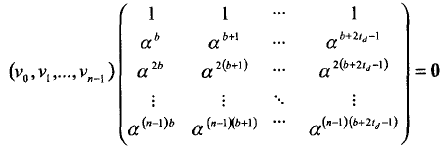
\includegraphics[scale=0.6]{chapter_2/img_08.png}
\end{center}
\end{figure}

Соответственно, проверочная матрица двоичного БЧХ кода имеет вид
\begin{figure}[htbp]
\begin{center}
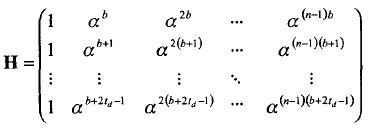
\includegraphics[scale=0.6]{chapter_2/img_09.png}
\end{center}
\end{figure}

Эта проверочная матрица обладает свойством: любая ее $2_{t_d} * 2_{t_d}$ подматрица является
\textit{матрицей Вандермонда}. Следовательно, любые $2_{t_d}$ столбцов матрицы линейно
независимы. Отсюда следует, что минимальное кодовое расстояние этого кода удовлетворяет
неравенству $d\ge 2_{t_d}+1$.

%%%%%%%%%%%%%%%%%%%%%%%%%%%%%%%%%%%%%%%%%%%%%%%%%%%%%%%%%%%%%%%%%%%%%%%%%%%%%%%%%%%%%%%%%%%
%%%%%%%%%%%%%%%%%%%%%%%%%%%%%%%%%%%%%%%%%%%%%%%%%%%%%%%%%%%%%%%%%%%%%%%%%%%%%%%%%%%%%%%%%%%
%%%%%%%%%%%%%%%%%%%%%%%%%%%%%%%%%%%%%%%%%%%%%%%%%%%%%%%%%%%%%%%%%%%%%%%%%%%%%%%%%%%%%%%%%%%
\subsection{Алгоритм кодирования БЧХ-кодом}
Кодирование БЧХ-кодом состоит из следующих операций:
\begin{enumerate}
  \item Получить вектор бит для кодирования.
  \item Преобразовать данный вектор в полином $m(x)$.
  \item Умножить полученный полином $m(x)$ на порождающий полином $g(x)$. В результате имеем полином $r(x)$.
  \item Преобразовать полученный полином $r(x)$ в вектор бит.
  \item Данный вектор бит явялется кодовым словом БЧХ-кода и передается в канал.
\end{enumerate}

%%%%%%%%%%%%%%%%%%%%%%%%%%%%%%%%%%%%%%%%%%%%%%%%%%%%%%%%%%%%%%%%%%%%%%%%%%%%%%%%%%%%%%%%%%%
%%%%%%%%%%%%%%%%%%%%%%%%%%%%%%%%%%%%%%%%%%%%%%%%%%%%%%%%%%%%%%%%%%%%%%%%%%%%%%%%%%%%%%%%%%%
%%%%%%%%%%%%%%%%%%%%%%%%%%%%%%%%%%%%%%%%%%%%%%%%%%%%%%%%%%%%%%%%%%%%%%%%%%%%%%%%%%%%%%%%%%%
\subsection{Общий алгоритм декодирования}
На Рис.~\ref{img_13} показана обобщенная структура декодера циклического кода. Синдром
$s(x)$ используется для определения полинома ошибок $e(x)$. Проблема декодирования равноценна
поиску полинома ошибок $e(x)$ по известному синдрому $s(x)$ .

\begin{figure}[htbp]
\begin{center}
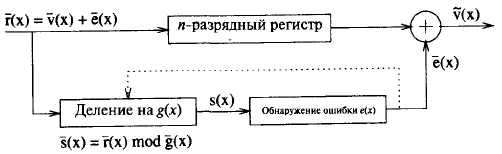
\includegraphics[scale=0.7]{chapter_2/img_13.png}
\end{center}
\caption{Обобщенная структура декодера циклического кода}
\label{img_13}
\end{figure}

%%%%%%%%%%%%%%%%%%%%%%%%%%%%%%%%%%%%%%%%%%%%%%%%%%%%%%%%%%%%%%%%%%%%%%%%%%%%%%%%%%%%%%%%%%%
%%%%%%%%%%%%%%%%%%%%%%%%%%%%%%%%%%%%%%%%%%%%%%%%%%%%%%%%%%%%%%%%%%%%%%%%%%%%%%%%%%%%%%%%%%%
%%%%%%%%%%%%%%%%%%%%%%%%%%%%%%%%%%%%%%%%%%%%%%%%%%%%%%%%%%%%%%%%%%%%%%%%%%%%%%%%%%%%%%%%%%%
\subsection{Алгоритм декодирования Берлекэмпа–Месси}
Декодирование БЧХ-кодов распадается на несколько задач. Это (1) вычисление синдромных компонент, (2) 
отыскание полинома локаторов ошибок, (3) отыскание самих локаторов ошибок как величин, обратных корням 
полинома локаторов ошибок, (4) определение величин ошибок. Архитектура БЧХ-декодера показана
на Рис.~\ref{img_11}.

\begin{figure}[htbp]
\begin{center}
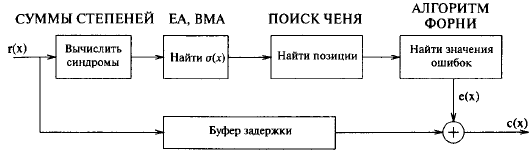
\includegraphics[scale=0.7]{chapter_2/img_11.png}
\end{center}
\caption{Архитектура БЧХ-декодера}
\label{img_11}
\end{figure}

Первоначальная версия алгоритма Берлекэмпа–Месси была изложена Берлекэмпом в 1968 году в качестве 
элемента конструкции декодера кодов Боуза–Чоудхудри–Хоквингема над конечным полем. Хотя в этой работе была 
указана возможность формулировки решаемой задачи с использованием понятия линейного регистра сдвига с 
обратной связью, алгоритм описывался исключительно в терминах полиномов и был весьма сложен для понимания. 
Спустя год Месси предложил свою интерпретацию алгоритма, как позволяющего строить линейный регистр сдвига 
минимальной длины, генерирующий заданную последовательность. Эта интерпретация оказалась полезной для более 
широкого распространения алгоритма, получившего название по имени этих двух ученых. В некоторых работах 
алгоритм излагается также с помощью непрерывных дробей и рациональной аппроксимации.

Данный алгоритм по числу операций в поле обладает высокой эффективностью и обычно рассматривается как 
итеративный процесс построения минимального линейного регистра сдвига с обратной связью. Особенностью данного 
регистра является то, что он генерирует заранее известную \emph{последовательность синдромов} $S_1, S_2, 
..., {S_2}_d$.

Алгоритм Берлекэмпа–Месси нацелен на построение многочлена $\sigma^{(l+1)}(x)$ наименьшей степени, который
удовлетворяет уравлению: $$\sum \limits_{j=0}^{l_i+1}S_{k-j}{\sigma_j}^{(i+1)}=0, l_i<k<i+1$$

Решение денной задачи эквивалентно условию, что многочен
$$\sigma^{(i+1)}(x)=1+{\sigma_1}^{(i+1)}x+\ldots+{\sigma_{l_i+1}}^{(i+1)}x^{l_{i+1}}$$

является многочленом обратной связи ЛРОС, который генерирует ограниченную последовательность синдромов.
Различие на $i$-й итерации определяется как
$$d_i=S_{i+1}+S_i\sigma_1^{(i)}+\ldots+S_{i-l_i+1}\sigma_{l_i}^{(i)}$$

является мерой соответствия синдромной последовательности и генерируемой ЛРОС и содержит корректирущий
множитель для вычисления $\sigma^{(i+1)}$ на следующей итерации. Существуют два случая:
\begin{enumerate}
\item Если $d_i=0$, то уравнение удовлетворяется неравенством.
$$\sigma{(i+1)}(x)=\sigma^1(x), l_{i+1}=l_i$$

\item Если $d\ne0$, то решение на следующей итерации имеет вид
$$\sigma^{(i+1)}(x)=\sigma^1(x)+d_i {d_m}^{-1}x^{t-m}\sigma^{(m)}(x)$$
$$l_{i+1}=max\{l_i, l_m+i-m\},$$

где является решением на $m$-й итерации такое, что $-1\le m<i$, $d_m\ne 0$, и разность $(m-l_m)$ максимальна.
Итеративное вычисление $\sigma^{(i+1)}(x)$ продолжается, пока не удовлетворится одно или оба условия: либо
$i\ge l_{i+1}+t_d-1$, либо $i=2t_d-1$.
\end{enumerate}
 
Начальные условия алгоритма:
$$\sigma^{(-1)}(x)=1, l_{-1}=0, d_{-1}=1$$
$$\sigma^{(0)}(x)=1, l_0=0, d_{0}=S_1.$$

Алгоритм Берлекэмпа–Месси можно рассматривать как итеративный процесс построения минимального линейного
регистра сдвига с обратной связью (ЛРОС), аналогично показанному на Рис.~\ref{img_12}, который
генерирует известную \textit{последовательность синдромов} $S_1, S_2, \ldots, S_{2t_d}$.

\begin{figure}[htbp]
\begin{center}
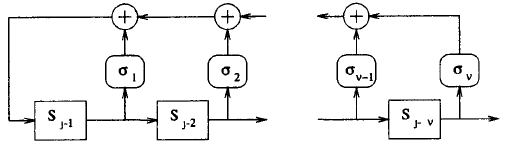
\includegraphics[scale=0.6]{chapter_2/img_12.png}
\end{center}
\caption{Архитектура БЧХ-декодера}
\label{img_12}
\end{figure}

%%%%%%%%%%%%%%%%%%%%%%%%%%%%%%%%%%%%%%%%%%%%%%%%%%%%%%%%%%%%%%%%%%%%%%%%%%%%%%%%%%%%%%%%%%%
%%%%%%%%%%%%%%%%%%%%%%%%%%%%%%%%%%%%%%%%%%%%%%%%%%%%%%%%%%%%%%%%%%%%%%%%%%%%%%%%%%%%%%%%%%%
%%%%%%%%%%%%%%%%%%%%%%%%%%%%%%%%%%%%%%%%%%%%%%%%%%%%%%%%%%%%%%%%%%%%%%%%%%%%%%%%%%%%%%%%%%%
\subsection{Решение ключевого уравнения}
%\begin{definition} 
%\deft{Ключевое уравнение для задачи исправления ошибок} --- уравнение вида 
%$$\Omega(x)=S(x)\lambda(x)mod x^{d-1}$$
%где $S(x)$ --- синдромный полином, а полиномы $\lambda(x)$ и $\Omega(x)$ должны быть определены в 
%процессе декодирования, $d$ --- конструктивное расстояние.
%\end{definition}
%
%Всякий метод решения ключевого уравнения при котором по заданному $S(x)$ отыскиваются полиномы $\lambda(x)$ 
%и $\Omega(x)$ такие, что $deg\lambda(x)=t, \Omega(x)=t-1, t\le(d-1)/2$, дает некоторый метод исправления
%ошибок кратности $t$.
Если кодер передает слово двоичного БЧХ-кода
$$C(x)=\sum\limits_{i=0}^{n-1} C_i x^i,$$

а шум в канале задается вектором
$$E(x)=\sum\limits_{i=0}^{n-1} E_i x^i,$$

то полученное слово записывается многочленом
$$R(x)=\sum\limits_{i=0}^{n-1} R_i x^i=\sum\limits_{i=0}^{n-1} C_i x^i+\sum\limits_{i=0}^{n-1} E_i x^i.$$

Для $j=1, 2, \ldots, 2t$ кодовое слово кратно минимальному многочлену элемента $\alpha^j$ и, следовательно,
$$R(\alpha^j)=0+\sum\limits_{i=0}^{n-1} E_i \alpha^{ji}=S_j,$$

где элементы поля Галуа $X_1, X_2, \ldots, X_e$ -- локаторы ошибок $E_i=1$. Так как
$S_j=R(\alpha^j)=r^{(\alpha^j)}(\alpha^j)$, где $r^j(x)$ -- остаток от деления $R(x)$ на минимальный
многочлен $M^{(j)}(x)$ элемента $\alpha^j(1\le j \le 2t)$. После вычисления $S_1, S_2, \ldots, S_{2t}$
основная задача декодера -- определить $X_1, X_2, \ldots, X_e$ из уравнений
$$\sum\limits_{i=1}^{e} X_i^j=S_j,  j=1, 2, \ldots, 2t.$$

В обшщем случае эта система имеет много решений, каждое из которых соответствует различным векторам
ошибок, лежащим в одном классе смежности по аддитивной группе кодовых слов. Декодер должен найти решение
с наимешьшим возможным числом $e$.

Для решения системы декодер сначала пытается определить коэффициенты многочлена локаторов ошибок.

\begin{definition} 
$$\sigma(z)=\prod\limits_{i=1}^{e}(1-X_i z)=1+\sum\limits_{j=1}^{e}\sigma_j z^j.$$
\end{definition}

Если многочлен $\sigma(z)$ уже найден декодером, то, используя процедуру Ченя, можно найти взаимные
корни для $\sigma(z)$. Наиболее тяжелая часть этой процедуры -- определение коэффициентов $\sigma_j$
по величинам $S_j$.

Для того чтобы найти зависимость между величинами $\sigma_j$ и $S_j$, введем производящую функцию
$$S(z)=\sum\limits_{i=1}^{\infty}S_j z^j=\sum\limits_{j=1}^{\infty}\sum\limits_{i=1}^{e}X_i^j z^j=
\sum\limits_{i=1}^{e}\frac{X_{i^z}}{1-X_{i^z}}.$$

После умножения на $\sigma(z)$ имеем
$$S(z)\sigma(z)=\sum\limits_{i=1}^{e}\frac{X_{i^z}}{1-X_{i^z}}\prod\limits_{j=1}^{e}(1-X_{i^z})=
\sum\limits_{i=1}^{e}X_(i^z)\prod\limits_{j\ne i}^{}(1-X_{i^z}).$$

Прибавив к обеим частям равенства $\sigma(z)$ получим
$$[1+S(z)]\sigma(z)=\sigma(z)+\sum\limits_{i=1}^{e}X_{i^z}\prod\limits_{j\ne i}^{}(1-X_{t^z}).$$

Определим многочлен $\omega(z)=\sum\limits_{k=0}^{e}\omega_k z^k$  спомощью равенства
$$\omega(z)=\sigma(z)+\sum\limits_{k=0}^{e}X_{i^z}\prod\limits_{j\ne i}^{}(1-X_{t^z}).$$

Тогда
$$[1+S(z)]\sigma(z)=\omega(z).$$

В общем случае декодеру известны коэффициенты только при первых $2t$ степенях $z$ в $S(z)$
и не известны коэффициенты $S_{2t+1}, S_{2t+2}, S_{2t+3}, \ldots .$ Иными словами, декодер
не знает $S(z)$, но знает $S(z)mod z^{2t+1}.$ Поэтому естественно ввести уравнение, которое
мы назовем \textit{ключевым}:

$$[1+S(z)]\sigma(z)=\omega(z)mod z^{2t+1}.$$

Из этого уравнения по заданному $S(z)$ нужно найти \textit{оба} многочлена $\sigma(z)$
и $\omega(z)$, степени которых не превосходят $e$, где $e$ -- число ошибок в канале.

Одна <<физическая интерпретация>> ключевого уравнения была предложена Месси. Перепишем
уравнение в виде
$$S_k+\sum\limits_{i=1}^{k-1}\sigma_i S_{k-i}+\sigma_k=\omega_k,$$

или в виде
$$S_k=\omega_k-\sum\limits_{i=1}^{k-1}\sigma_iS_{k-i}-\sigma_k.$$

Последнее равенство задает $k$-й выход регистров сдвига, приведенных на Рис.~\ref{img_06} и Рис.~\ref{img_07}.
Обратные связи которых соответствуют многочлену $\sigma(z)$, а начальное состояние ячеек --
многочлену $\omega(z)$. 
\begin{figure}[htbp]
\begin{center}
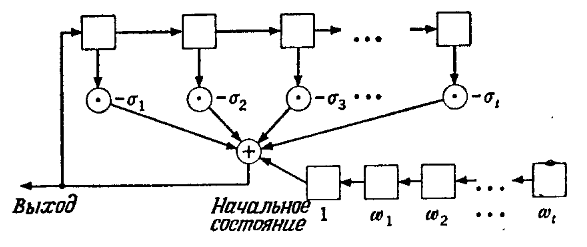
\includegraphics[scale=0.6]{chapter_2/img_06.png}
\end{center}
\caption{Интерпретация ключевого уравнения с помощью РОС}
\label{img_06}
\end{figure}

Это позволяет интерпретировать ключевое уравнение как математическую постановку задачи синтеза регистра
с обратной связью: по заданной выходной последовательности $1+S(z)$ необходимо определить обратные
связи $\sigma(z)$ и начальное состояние $\omega(z)$ кратчайшего регистра сдвига с выходной последовательностью
$1+S(z)$.

В задаче декодирования двоичных БЧХ-кодов реальный интерес представляет многочлен $\sigma(z)$, а не
многочлен $\omega(z)$. Однако это же ключевое уравнение возникает и в некоторых других приложениях.

\begin{figure}[htbp]
\begin{center}
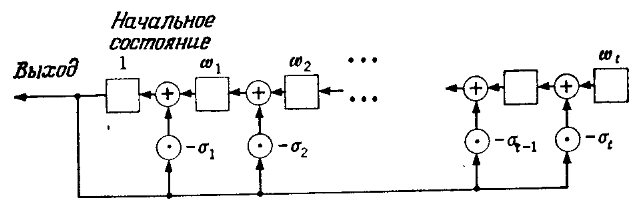
\includegraphics[scale=0.6]{chapter_2/img_07.png}
\end{center}
\caption{Другая интерпретация ключевого уравнения с помощью РОС}
\label{img_07}
\end{figure}

%%%%%%%%%%%%%%%%%%%%%%%%%%%%%%%%%%%%%%%%%%%%%%%%%%%%%%%%%%%%%%%%%%%%%%%%%%%%%%%%%%%%%%%%%%%
%%%%%%%%%%%%%%%%%%%%%%%%%%%%%%%%%%%%%%%%%%%%%%%%%%%%%%%%%%%%%%%%%%%%%%%%%%%%%%%%%%%%%%%%%%%
%%%%%%%%%%%%%%%%%%%%%%%%%%%%%%%%%%%%%%%%%%%%%%%%%%%%%%%%%%%%%%%%%%%%%%%%%%%%%%%%%%%%%%%%%%%
\subsection{Вычисление синдромов}
Синдромы вычисляются как значения принятого полнинома в нулях кода
\footnote{Для двоичных БЧХ кодов справедливо равенство $S_{2i}=S_i^2$, которое
позволяет сократить объем вычислений.}
$$S_i=r(\alpha^i), i=b, b+1, \ldots, b+2t_d -1$$

Вычисление синдромов может быть реализовано аппаратно. На Рис.~\ref{img_10} показан
пример схемы аппаратного вычисления синдрома.
\begin{figure}[htbp]
\begin{center}
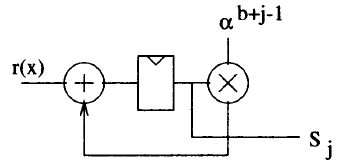
\includegraphics[scale=0.6]{chapter_2/img_10.png}
\end{center}
\caption{Пример вычисления синдрома}
\label{img_10}
\end{figure}

%%%%%%%%%%%%%%%%%%%%%%%%%%%%%%%%%%%%%%%%%%%%%%%%%%%%%%%%%%%%%%%%%%%%%%%%%%%%%%%%%%%%%%%%%%%
%%%%%%%%%%%%%%%%%%%%%%%%%%%%%%%%%%%%%%%%%%%%%%%%%%%%%%%%%%%%%%%%%%%%%%%%%%%%%%%%%%%%%%%%%%%
%%%%%%%%%%%%%%%%%%%%%%%%%%%%%%%%%%%%%%%%%%%%%%%%%%%%%%%%%%%%%%%%%%%%%%%%%%%%%%%%%%%%%%%%%%%
\subsection{Граница Синглтона}
\textbf{Определение}

Граница Синглтона (названная в честь Р. К. Синглтона) устанавливает предел мощности кода $C$ 
с символами из поля $\mathbb{F}_q$ длины $n$ и минимального расстояния Хэмминга $d$.  

Пусть $A_q(n,d)$ обозначает максимально возможную мощность $q$-ичного кода длины $n$
($q$-ичный код — это код над полем из $q$ элементов). Пусть минимальное расстояние Хэмминга
между двумя словами кода будет $d$, то есть $\mathrm D_H(w,\;w')\geqslant d$ для любых двух
кодовых слов $w$ и $w'$. 

Тогда : $A_q(n,\;d)\leqslant q^{n-d+1}.$

\textbf{Доказательство}

В первую очередь заметим, что верхняя граница максимальной мощности любого $q$-ичного кода
длины $n$ равняется $q^n$, так как каждый компонент данного кодового слова может принимать
одно из $q$ разных значений независимо от других компонентов.

Пусть $C$ является $q$-ичным кодом. Тогда все слова $c \in C$ в кодe отличны друг от друга.
Если мы сотрём первые $d-1$ символов каждого слова, тогда все оставшиеся кодовые слова должны
оставаться разными, так как расстояние Хэмминга между словами кода $C$ по меньшей мере $d$.
Следовательно мощность кода после удаления $d-1$ символов осталась прежней.

Длина нового кода
$$n-(d-1)=n-d+1,$$

и следовательно максимально возможной мощностью такого кода является $q^{n-d+1}.$

Отсюда следует верхняя граница мощности и для изначального кода
$$A_q(n,\;d)\leqslant q^{n-d+1}.$$

\textbf{Линейные коды}

В случае с линейными кодами можно записать границу Синглтона как
$$q^k\leqslant q^{n-d+1}$$

или
$$k\leqslant n-d+1.$$

Линейные коды, для которых выполняется равенство $k=n-d+1$, называются \textit{разделимыми
кодами с максимальным расстоянием} или кодами МДР. Известными представителями этого семейства
кодов являются \textit{код Рида — Соломона} и коды, образуемые из него.

%%%%%%%%%%%%%%%%%%%%%%%%%%%%%%%%%%%%%%%%%%%%%%%%%%%%%%%%%%%%%%%%%%%%%%%%%%%%%%%%%%%%%%%%%%%
%%%%%%%%%%%%%%%%%%%%%%%%%%%%%%%%%%%%%%%%%%%%%%%%%%%%%%%%%%%%%%%%%%%%%%%%%%%%%%%%%%%%%%%%%%%
%%%%%%%%%%%%%%%%%%%%%%%%%%%%%%%%%%%%%%%%%%%%%%%%%%%%%%%%%%%%%%%%%%%%%%%%%%%%%%%%%%%%%%%%%%%
\section{Сверточные коды}

\begin{definition} 
\deft{Сверточные кодирование} --- метод кодирования, при котором каждый символ входной последовательности, 
состоящей из $k$ битов, преобразуется в $n$-битовый кодированный поток данных. Внесение избыточности и 
соответственное увеличение скорости передачи в $n/k$ раз, позволяет повысить помехоустойчивость, особенно в 
каналах с одиночными ошибками.
\end{definition}

\subsection{Алгоритм кодирования сверточным кодом}
Алгоритм основан на работе сверточного кодера. Кодер имеет набор входов и выходов. Символы информационной
последовательности поступают на вход кодера и попадают в регистр сдвига с обратной связью. В результате
выполения операции сдвига на выходах кодера появляются выходные символы, которые и формируют кодовые слова.

Сверточный кодер представлен на Рис.~\ref{img_02}.

\begin{figure}[htbp]
\begin{center}
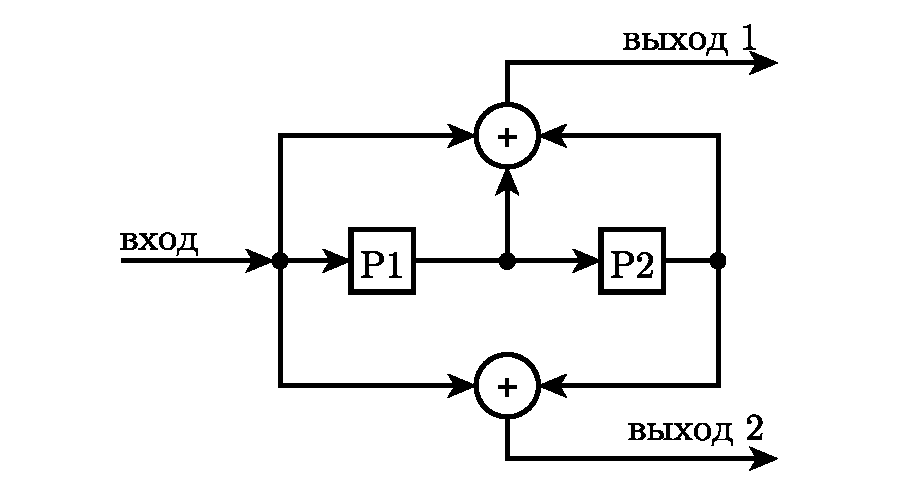
\includegraphics[scale=0.6]{chapter_2/img_02.pdf}
\end{center}
\caption{Сверточный кодер}
\label{img_02}
\end{figure}

%%%%%%%%%%%%%%%%%%%%%%%%%%%%%%%%%%%%%%%%%%%%%%%%%%%%%%%%%%%%%%%%%%%%%%%%%%%%%%%%%%%%%%%%%%%
%%%%%%%%%%%%%%%%%%%%%%%%%%%%%%%%%%%%%%%%%%%%%%%%%%%%%%%%%%%%%%%%%%%%%%%%%%%%%%%%%%%%%%%%%%%
%%%%%%%%%%%%%%%%%%%%%%%%%%%%%%%%%%%%%%%%%%%%%%%%%%%%%%%%%%%%%%%%%%%%%%%%%%%%%%%%%%%%%%%%%%%
\subsection{Алгоритм Витерби}
Классическим методом коррекции ошибок, по праву считавшимся лучшим в течение нескольких десятилетий, является 
декодер Витерби, применяемый для декодирования сверточных кодов. Данный алгоритм является оптимальным и легко 
реализуемым для коротких сверточных кодов. В связи с этим сверточные коды, декодируемые с помощью алгоритма 
Витерби, применяются в большинстве стандартов систем передачи данных, например, в беспроводных сетях 
стандартов IEEE 802.11, IEEE 802.16, дальней космической связи CCSDS, спутниковой связи TIA-1008 и др. 
Использование длинных (с конструктивной длиной более 9) и потенциально более эффективных кодов в декодере 
Витерби представляется нецелесообразным из-за экспоненциального роста сложности его реализации от длины кода. 
Поэтому долгое время усилия многих специалистов были направлены на разработку алгоритмов декодирования, 
которые способны эффективно декодировать длинные коды при небольшой сложности реализации.

В основе алгоритм Витерби лежит принцип максимума правдоподобия. В процессе декодирования кодового слова
декодер Витерби находит кодовую последовательность, ближайшую к принятой. 

\begin{enumerate}
\item Вычисление метрик рёбер решётки. Метрика ребра решётки на вычисляется как Хэмминговое расстояние
между меткой ребра и двоичной последовательностью на входе декодера. Расстояние между последовательностями
по Хэммингу --- количество различающихся битов в последовательностях.
\item Прибавить, сравнить, выбрать.
Для каждого состояния и соответствующей пары рёбер, входящих в данное состояние из двух возможных
предшествующих, вычислить и сравнить следующие суммы. Выбрать ребро с меньшей суммой.
\item Декодирование символов.
Вычислить декодируемый символ и записать его в буфер накопленной последовательности. При этом выдать
ранее сохраненный символ на выход декодера.
\end{enumerate}

Особенностью Декодер Витерби является то, что при последовательном декодировании при возникновении
ошибок в канале метрики путей растут. Для устранения этого недостатка выполняется процедура
нормализации метрик. Существует два способа нормализации метрик: пороговый и модулярный.

Пример декодирования кодового слова с использованием алгоритма Витерби приведен на на Рис.~\ref{img_03}.

\begin{figure}[htbp]
\begin{center}
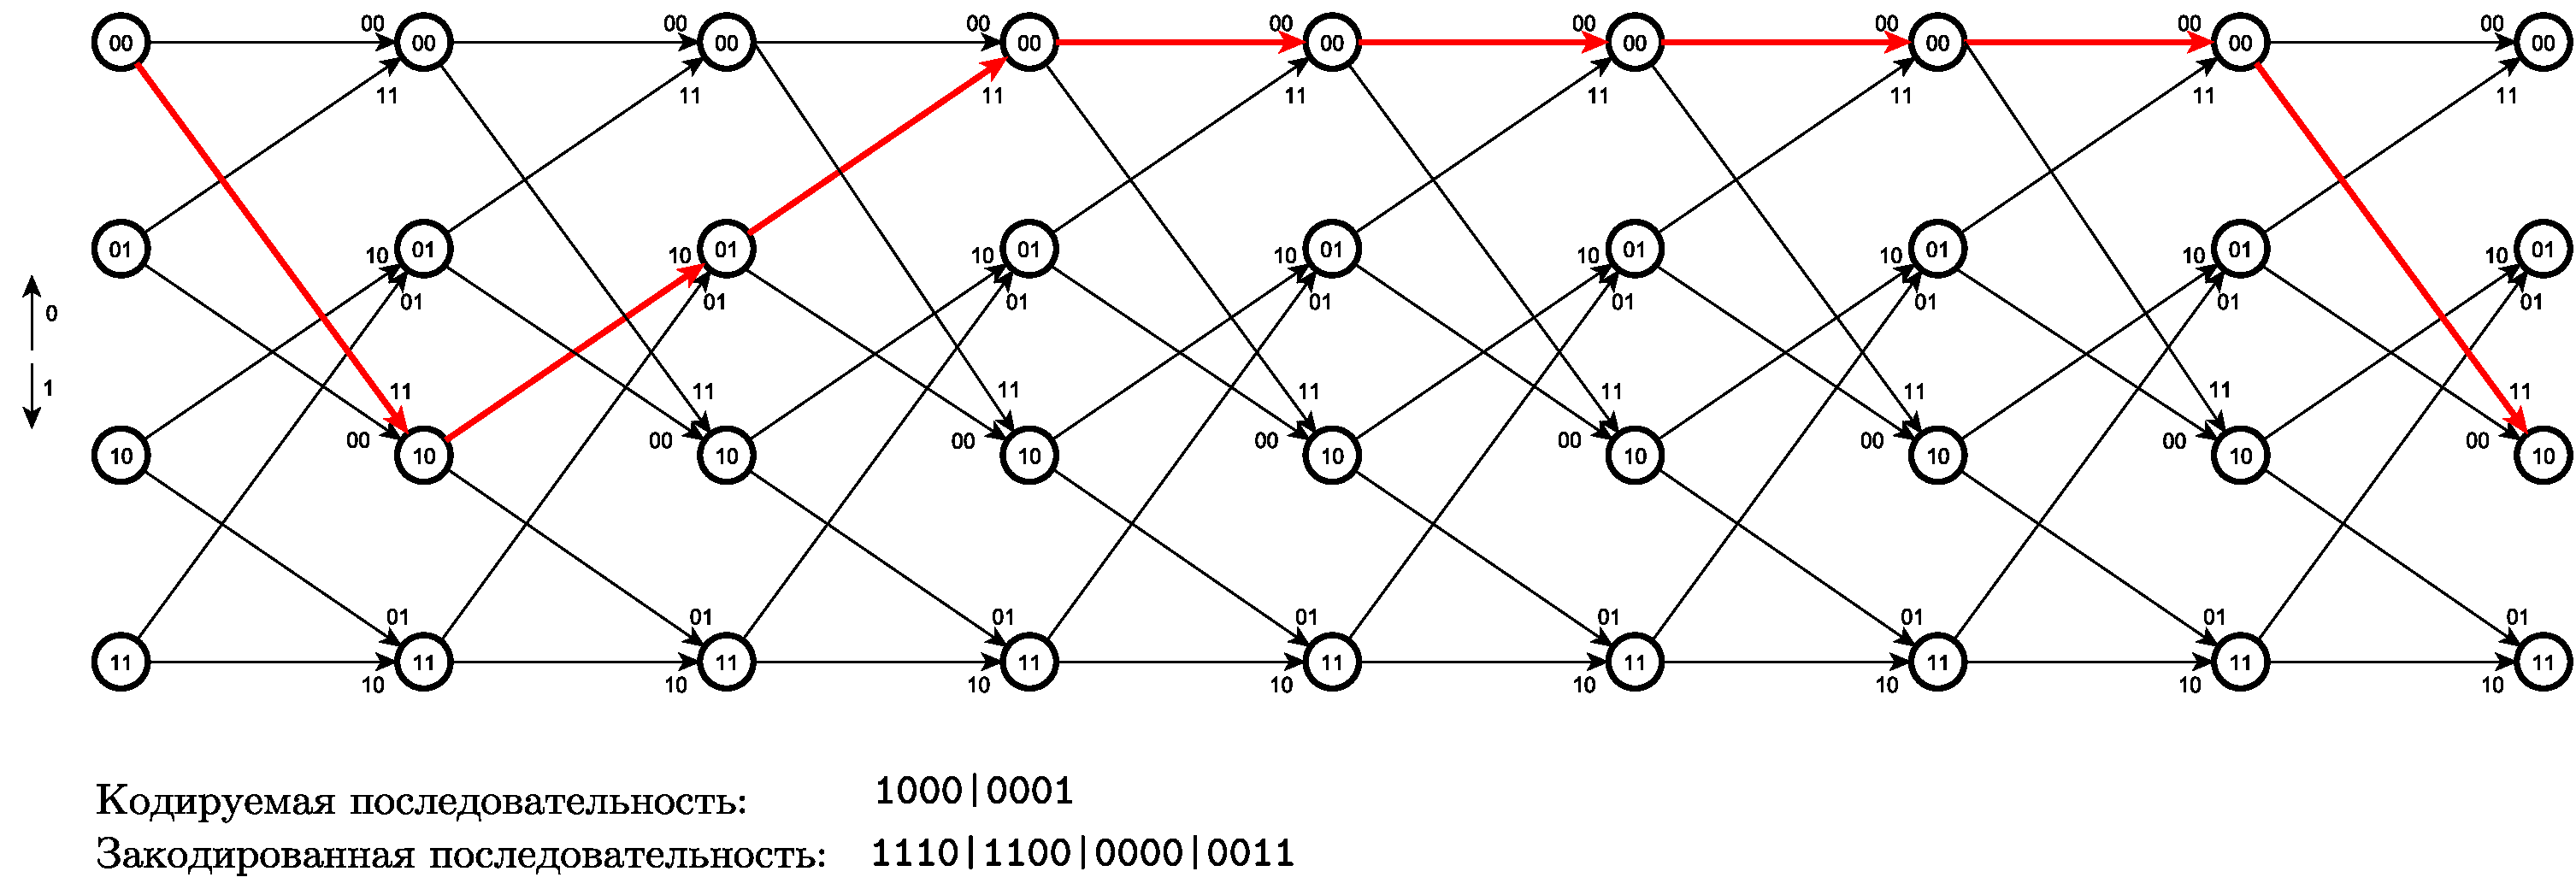
\includegraphics[scale=0.3]{chapter_2/img_03.pdf}
\end{center}
\caption{Декодирование кодового слова с использованием алгоритма Витерби}
\label{img_03}
\end{figure}

%%%%%%%%%%%%%%%%%%%%%%%%%%%%%%%%%%%%%%%%%%%%%%%%%%%%%%%%%%%%%%%%%%%%%%%%%%%%%%%%%%%%%%%%%%%
%%%%%%%%%%%%%%%%%%%%%%%%%%%%%%%%%%%%%%%%%%%%%%%%%%%%%%%%%%%%%%%%%%%%%%%%%%%%%%%%%%%%%%%%%%%
%%%%%%%%%%%%%%%%%%%%%%%%%%%%%%%%%%%%%%%%%%%%%%%%%%%%%%%%%%%%%%%%%%%%%%%%%%%%%%%%%%%%%%%%%%%
\section{Каскадные коды}
Каскадные коды используются в практике передачи дискретных сигналов в качестве методов реализации кодов 
большой длины и высокой корректирующей способности. Эта цель может быть достигнута применением нескольких 
ступеней кодирования; наибольшее распространение получили две ступени кодирования различными кодами, например 
по схеме, показанной на Рис.~\ref{img_04}.

\begin{figure}[htbp]
\begin{center}
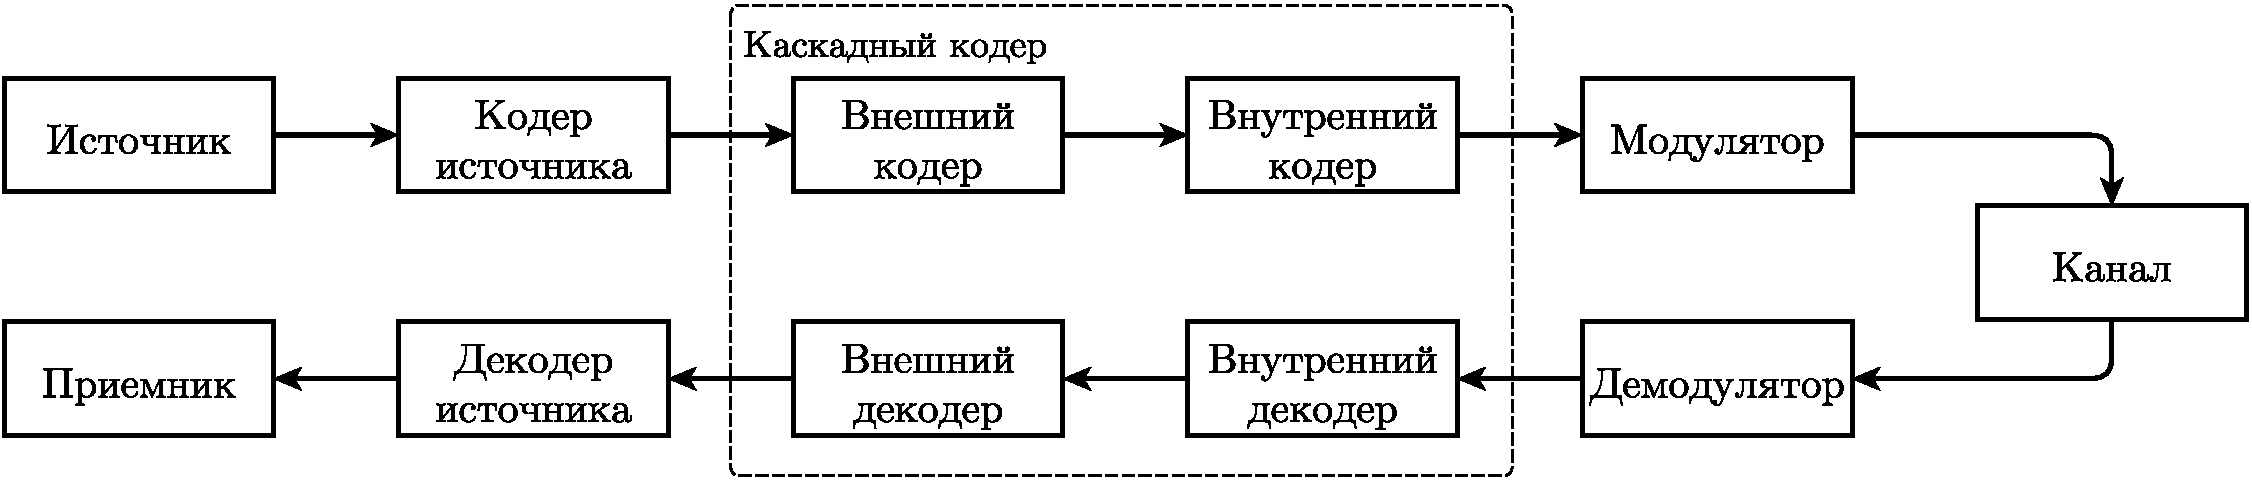
\includegraphics[scale=0.4]{chapter_2/img_04.pdf}
\end{center}
\caption{Cистема передачи информации при использовании каскадного кодирования}
\label{img_04}
\end{figure}

Поступающие от источника сообщений данные разбиваются на блоки из $К$ недвоичных ($m$-ичных) символов, 
содержащие $k$ информационных элементов ($k=km$), которые кодируются недвоичным $(n, k)$кодом. Очевидно, что 
каждый коэффициент $(n, k )$ кода cодержит $m$ двоичных элементов. Последовательность $(n, k)$ кода, 
состоящая из $n_1=nm$ двоичных элементов поступает на внутренний кодер, где разбивается на $m$-элементные 
блоки, которые кодируются внутренним $(n_2, m)$ кодом. Число кодовых комбинаций $N=K+R$, поэтому на выходе 
внутреннего кодера число двоичных элементов будет $n=n_2*N$.

%%%%%%%%%%%%%%%%%%%%%%%%%%%%%%%%%%%%%%%%%%%%%%%%%%%%%%%%%%%%%%%%%%%%%%%%%%%%%%%%%%%%%%%%%%%
%%%%%%%%%%%%%%%%%%%%%%%%%%%%%%%%%%%%%%%%%%%%%%%%%%%%%%%%%%%%%%%%%%%%%%%%%%%%%%%%%%%%%%%%%%%
%%%%%%%%%%%%%%%%%%%%%%%%%%%%%%%%%%%%%%%%%%%%%%%%%%%%%%%%%%%%%%%%%%%%%%%%%%%%%%%%%%%%%%%%%%%
\subsection{Получение каскадных кодов}
Схема системы передачи информации, используемая для анализа кодов в данной работе представлена на
Рис.~\ref{img_05}.

\begin{figure}[htbp]
\begin{center}
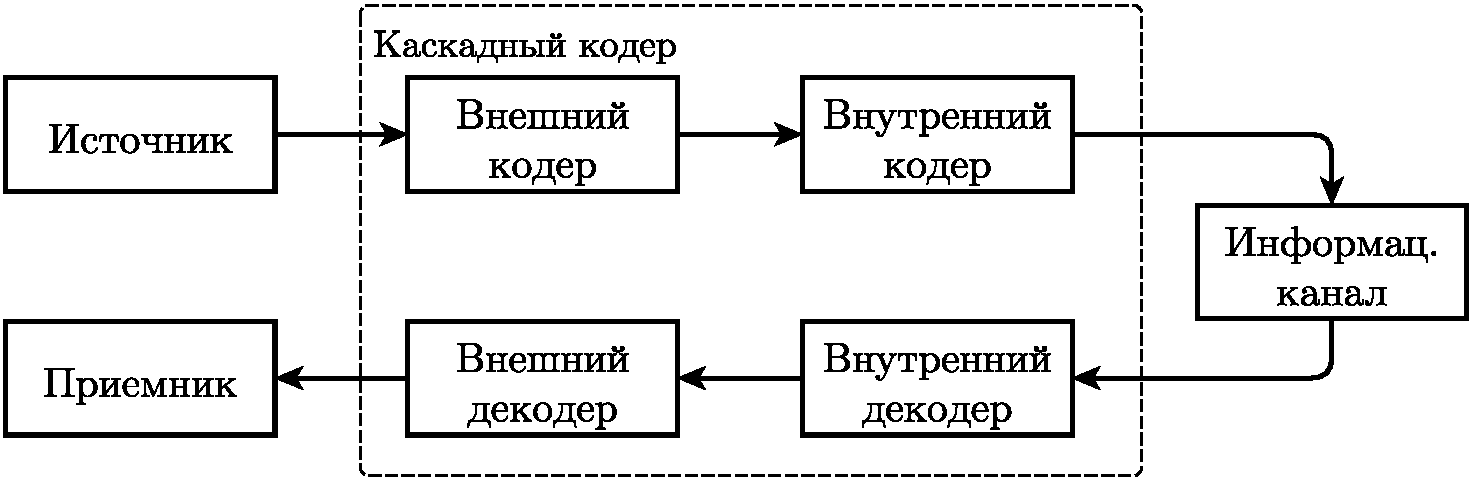
\includegraphics[scale=0.4]{chapter_2/img_05.pdf}
\end{center}
\caption{Cистема передачи информации для анализа кодов}
\label{img_05}
\end{figure}

В данной работе внешним кодером выступает БЧХ-кодер, который генерирует кодовое слово БЧХ-кода c параметрами 
$(15, 5, 7 )$. Установлено, что данный код гарантированно исправляет ошибки в количестве $t\le3$. Указанное 
слово поступает на вход внутреннего кодера, которым является сверточный кодер. Он принимает кодовое слово БЧХ
-кода и кодирует его в слово сверточного кода с параметрами $(2, 1)$. На выходе получаем кодовые слова 
сверточного кода, которые поступают в модулятор. В данной работе модулятор не используется по причине 
акцента внимания на анализ кодов. Таким образом, кодовые слова сверточного кода поступают в информационный 
канал, где происходит их искажение.

%%%%%%%%%%%%%%%%%%%%%%%%%%%%%%%%%%%%%%%%%%%%%%%%%%%%%%%%%%%%%%%%%%%%%%%%%%%%%%%%%%%%%%%%%%%
%%%%%%%%%%%%%%%%%%%%%%%%%%%%%%%%%%%%%%%%%%%%%%%%%%%%%%%%%%%%%%%%%%%%%%%%%%%%%%%%%%%%%%%%%%%
%%%%%%%%%%%%%%%%%%%%%%%%%%%%%%%%%%%%%%%%%%%%%%%%%%%%%%%%%%%%%%%%%%%%%%%%%%%%%%%%%%%%%%%%%%%
\subsection{Декодирование каскадных кодов}
При декодировании каскадного кода выполняется ряд обратных кодированию процедур. Так, при демодуляции на 
удаленной стороне имеем кодовое слово сверточного кода. Данное слово декодируется сверточным декодером, 
который построен на основе алгоритма Витерби. В результате декодирования нескольких кодовых слов имеем 
кодовое слово БЧХ-кода, которое подается на вход БЧХ-декодеру. В результате декодирования данного слова 
имеем исходные данные, то есть данные сгенерированные кодером источника.  Очевидно, что принцип каскадного 
декодирования аналогичен действию получателя искаженной телеграммы. Так, если искажены буквы в словах (
независимые ошибки в канале), то они могут быть обнаружены и исправлены с помощью других букв того же слова (
внутреннее кодирование решает эту задачу), а если же отдельные слова искажены до неузнаваемости ( 
группирующиеся ошибки пакеты), то обнаруженное наличие таких ошибок и тем более их исправление возможно 
только с помощью других слов предложения или текста в целом (внешнее кодирование). В рассмотренной аналогии 
основу внутреннего кода составляет избыточность за счет связей между буквами в словах, а внешнего кода за 
счет связей слов в предложении.